% ------------------------------------------------------------------
\renewcommand{\thisweek}{MATH327 Week 9}
\renewcommand{\moddate}{Last modified 24 Apr.~2021}
\setcounter{section}{9}
\setcounter{subsection}{0}
\phantomsection
\addcontentsline{toc}{section}{Week 9: Quantum gases of fermions}
\section*{Week 9: Quantum gases of fermions}
\subsection{Non-relativistic ideal fermion gas}
This week we wrap up our applications of the grand-canonical ensemble to investigate ideal gases of non-interacting particles.
We again take the quantum statistical approach of defining micro-states by summing over the possible occupation numbers $n_{\ell}$ for each energy level $\cE_{\ell}$ with energy $E_{\ell}$.
In contrast to the bosonic case considered last week, we now focus on quantum gases of fermions, where the only possible occupation numbers are $n_{\ell} = 0$ and $1$, since the Pauli exclusion principle prevents multiple identical fermions from occupying the same energy level.

In \secref{sec:fermi} we derived the grand-canonical partition function (\eq{eq:partfunc_FD}) that defines quantum Fermi--Dirac statistics for such systems of non-interacting fermions,
\begin{equation*}
  \ZFD(\be, \mu) = \prod_{\ell = 0}^L \left[1 + e^{-\be (E_{\ell} - \mu)}\right],
\end{equation*}
for inverse temperature $\be = 1 / T$ and chemical potential $\mu$.
Recall that it is possible for systems of fermions to have any value for the chemical potential (either positive or negative), in contrast to the systems of bosons we considered last week.
From the corresponding grand-canonical potential,
\begin{equation*}
  \Phi_{\text{FD}} = -T \sum_{\ell = 0}^L \log\left[1 + e^{-\be (E_{\ell} - \mu)}\right]
\end{equation*}
we can determine the large-scale properties of the system, including its average internal energy $\vev{E}$, average particle number $\vev{N}$, entropy $S$, and pressure $P$, along with the equation of state relating these quantities.

A concrete calculation requires specifying the energy levels of the particles that compose the gas, and the degeneracies of those energy levels.
Let's begin this week by considering non-relativistic particles of the sort we previously analyzed in \secref{sec:regulate}.
In a volume $V = L^3$, the energy levels are defined by the non-zero quantized energies
\begin{align*}
  E(k) & = \frac{p^2}{2m} = \frac{\hbar^2 \pi^2}{2mL^2}\left(k_x^2 + k_y^2 + k_z^2\right) &
  k_{x, y, z} & = 1, 2, \cdots.
\end{align*}
In addition to the usual degeneracies coming from permutations of $(k_x, k_y, k_z)$ that we discussed in previous weeks, for each distinct $\vec k$ typical fermions such as electrons have two degenerate energy levels with the same energy.
This factor of $2$ has a different origin compared to the double degeneracy discussed for photons last week.
Rather than worry about the physical origins of this behaviour, in both cases we simply incorporate this given information into our ansatz. % TODO: Could mention spin...

The grand-canonical potential for an ideal gas of non-relativistic fermions is therefore
\begin{equation*}
  \Phi_{\text{f}} = T \sum_{\ell = 0}^L \log\left[1 + e^{-\be (E_{\ell} - \mu)}\right] = 2T \sum_{\vec k} \log\left[1 + \exp\left(-\frac{\hbar^2 \pi^2 k^2}{2mL^2 T} + \frac{\mu}{T}\right)\right].
\end{equation*}
We can again proceed by considering the gas in a large volume and approximating the sum over discrete integer $k_{x, y, z}$ by integrals over continuous real $\khat_{x, y, z}$:
\begin{equation*}
  \Phi_{\text{f}} \approx 2T \int d\khat_x d\khat_y d\khat_z \log\left[1 + \exp\left(-\frac{\hbar^2 \pi^2 \khat^2}{2mL^2 T} + \frac{\mu}{T}\right)\right].
\end{equation*}
Converting to spherical coordinates and carrying out the angular integrations over the $\frac{\pi}{2}$ solid angle of the octant of the sphere with $k_{x, y, z} > 0$, we have
\begin{equation*}
  \Phi_{\text{f}} \approx \pi T \int_0^{\infty} d\khat \; \khat^2 \log\left[1 + \exp\left(-\frac{\hbar^2 \pi^2 \khat^2}{2mL^2 T} + \frac{\mu}{T}\right)\right].
\end{equation*}
In the same spirit as the change of variables we carried out last week, to integrate over photon frequencies $\om = \Eph / \hbar$, we will now change variables to integrate over the fermion energy:
\begin{align*}
  E = \frac{\hbar^2 \pi^2}{2mL^2}\khat^2 \quad \lra \quad \khat & = \frac{L\sqrt{m}}{\pi \hbar} \sqrt{2E} \cr
                                                         d\khat & = \frac{L\sqrt{m}}{\pi \hbar} \frac{dE}{\sqrt{2E}}.
\end{align*}
Plugging this in produces
\begin{align}
  \Phi_{\text{f}} & \approx \pi T \left(\frac{L^3 m^{3 / 2}}{\pi^3 \hbar^3}\right) \int_0^{\infty} dE \frac{2E}{\sqrt{2E}} \log\left[1 + e^{-\be(E - \mu)}\right] \cr
                  & = \frac{\sqrt{2 m^3} VT}{\pi^2 \hbar^3} \int_0^{\infty} dE \sqrt{E} \log\left[1 + e^{-\be(E - \mu)}\right]. \label{eq:fermi_grand}
\end{align}
recognizing $L^3 = V$.

With this grand-canonical potential derived, we just need to take the appropriate derivatives to determine the thermodynamics and equation of state for non-relativistic fermions.
When doing so, we'll focus on the low-temperature regime where we expect quantum Fermi--Dirac statistics to differ significantly from the classical case we considered back in \secref{sec:regulate}.
As we saw in \secref{sec:quantum_classical}, at high temperatures (with large negative chemical potential) the classical approach provides a good approximation to the true quantum physics.
% TODO: Low temperatures provide a significant simplification, which is why we only consider that regime this week
% ------------------------------------------------------------------



% ------------------------------------------------------------------
\subsection{Low-temperature equation of state}
Rather than the average internal energy $\vev{E}_{\text{f}}$, it will prove profitable to first analyze the average particle number
\begin{equation*}
  \vev{N}_{\text{f}} = -\pderiv{}{\mu} \Phi_{\text{f}}
\end{equation*}
coming from the grand-canonical potential for non-relativistic fermions, \eq{eq:fermi_grand}.
In analogy to the Planck spectrum we derived for the photon gas last week, we first express the particle number density as an integral over energies,
\begin{equation*}
  \frac{\vev{N}_{\text{f}}}{V} = \frac{\sqrt{2m^3}}{\pi^2 \hbar^3} \int_0^{\infty} F(E) \sqrt{E} \; dE,
\end{equation*}
where the function $F(E)$ is known as the Fermi function.
In contrast to the Planck spectrum, all the constant factors are kept separate from $F(E)$:
\begin{align}
  \frac{\vev{N}_{\text{f}}}{V} & = \frac{\sqrt{2m^3} T}{\pi^2 \hbar^3} \int_0^{\infty} dE \sqrt{E} \pderiv{}{\mu} \log\left[1 + e^{-\be(E - \mu)}\right] \cr
                               & = \frac{\sqrt{2m^3}}{\pi^2 \hbar^3} \int_0^{\infty} \frac{1}{e^{\be(E - \mu)} + 1} \sqrt{E} \; dE = \frac{\sqrt{2m^3}}{\pi^2 \hbar^3} \int_0^{\infty} F(E) \sqrt{E} \; dE. \label{eq:N_fermi}
\end{align}
This allows the Fermi function to closely resemble the average occupation numbers $\vev{n_{\ell}}$ we computed in \secref{sec:quantum_classical}:
\begin{equation}
  F(E) = \frac{1}{e^{\be(E - \mu)} + 1}.
\end{equation}

As usual in the grand-canonical approach, the average particle number and Fermi function depend on both the inverse temperature \be and the chemical potential $\mu$.
Expressing $F(E)$ in terms of the dimensionless ratios $E / \mu$ and $T / \mu$,
\begin{equation*}
  F(E) = \frac{1}{\exp\left[\frac{E - \mu}{T}\right] + 1} = \frac{1}{\exp\left[\frac{\mu}{T}\left(\frac{E}{\mu} - 1\right)\right] + 1} = \frac{1}{\left(\exp\left[\frac{E}{\mu} - 1\right]\right)^{\mu / T} + 1},
\end{equation*}
we can highlight the two main features of the figure below, which plots the Fermi function against $E / \mu$ for various temperatures $T / \mu$.

\begin{center}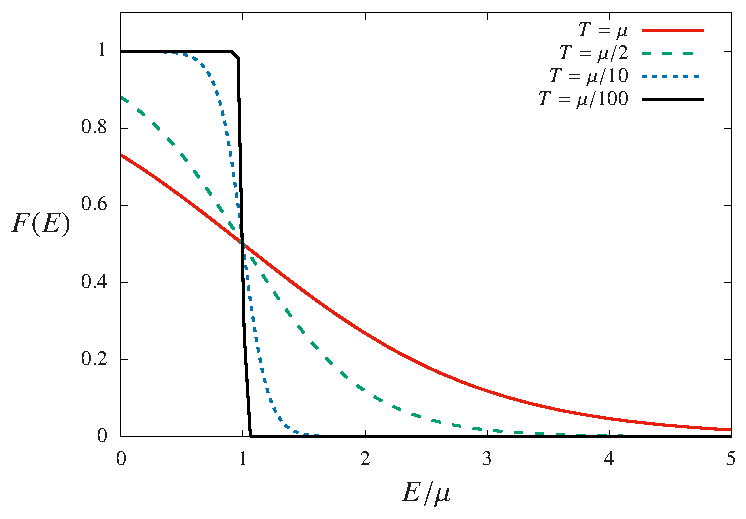
\includegraphics[width=\textwidth]{figs/week09_dist.pdf}\end{center}

First, we can see that the point $E = \mu$, where $F(E) = 1 / 2$ for any non-zero temperature, is a threshold at which the behaviour of the Fermi function changes.
For larger energies $E > \mu$, the exponential factor $\exp\left[\frac{E}{\mu} - 1\right] > 1$ and drives $F(E) \to 0$ as the energy increases.
For smaller energies $E < \mu$, the exponential factor $\exp\left[\frac{E}{\mu} - 1\right] < 1$ and vanishes as the energy decreases, leaving $F(E) \to 1$.
These two asymptotic limits reflect the possible energy level occupation numbers for fermions, $n_{\ell} = 0$ and $1$.
Second, smaller temperatures cause much more rapid approach to these two limits, with the exponential factor either enhanced (if $E > \mu$) or suppressed (if $E < \mu$) by a power $\mu / T \gg 1$.
Therefore, for small temperatures $T \ll \mu$, we can simplify our calculations by approximating the Fermi function as a step function,
\begin{equation}
  \label{eq:Fermi_step}
  F(E) \approx \left\{\begin{array}{l}1 \qquad \mbox{for } \ E < \mu \\
                                      0 \qquad \mbox{otherwise}\end{array}\right. .
\end{equation}
Using this approximation, what is the resulting particle number density?
\begin{mdframed}
  $\displaystyle \frac{\vev{N}_{\text{f}}}{V} = \frac{\sqrt{2m^3}}{\pi^2 \hbar^3} \int_0^{\infty} F(E) \sqrt{E} \; dE = $ \\[100 pt]
\end{mdframed}

You should find a result proportional to $\mu^{3 / 2}$ but independent of $T$.
The temperature independence can be understood by viewing this as the leading-order term in an expansion in the small temperature (known as a \textit{Sommerfeld expansion}, named after \href{https://en.wikipedia.org/wiki/Arnold_Sommerfeld}{Arnold Sommerfeld}).
The $\mu^{3 / 2}$ dependence on the chemical potential is also what we would predict even without doing the detailed calculation.
The step function in \eq{eq:Fermi_step} corresponds to a single fermion occupying each and every energy level with $E_{\ell} < \mu$, while all energy levels with $E_{\ell} > \mu$ are unoccupied.
Since $E(k) \propto k^2$, summing over all $k_{x, y, z}$ corresponds to computing (a portion of) the volume of a sphere of radius $r = \sqrt{\mu}$, which is proportional to $r^3 = \mu^{3 / 2}$ as we found directly above.
If we were to invert this relation, we would obtain the so-called \textbf{Fermi energy} as a function of the particle number density,
\begin{equation}
  \label{eq:Fermi_energy}
  E_F = \mu = \frac{\hbar^2}{2m}\left(\frac{3\pi^2 \vev{N}_{\text{f}}}{V}\right)^{2 / 3}.
\end{equation}

Now we can consider the average energy density of the non-relativistic fermion gas at low temperatures.
Rather than taking another derivative of the grand-canonical potential, we can note from \eq{eq:total_energy_levels} and from our work on the photon gas last week that
\begin{equation}
  \frac{\vev{E}_{\text{f}}}{V} = \frac{\sqrt{2m^3}}{\pi^2 \hbar^3} \int_0^{\infty} E \; F(E) \sqrt{E} \; dE.
\end{equation}
That is, instead of simply counting the number of fermions in the system, we need to add up their energies, introducing an extra factor of $E$ compared to \eq{eq:N_fermi}.
Still using the low-temperature step-function approximation for the Fermi function in \eq{eq:Fermi_step}, what is the average energy density?
\begin{mdframed}
  $\displaystyle \frac{\vev{E}_{\text{f}}}{V} = \frac{\sqrt{2m^3}}{\pi^2 \hbar^3} \int_0^{\infty} F(E) E^{3 / 2} \; dE = $ \\[100 pt]
\end{mdframed}

You should find
\begin{equation}
  \label{eq:fermi_E_N}
  \vev{E}_{\text{f}} = \frac{3}{5} \mu \vev{N}_{\text{f}},
\end{equation}
which means that the average energy of the fermions in a low-temperature ideal gas is $3 / 5$ the Fermi energy $E_F = \mu$.
In particular, because this result is also independent of the temperature, we find that non-interacting quantum fermions retain a positive energy even as the temperature approaches absolute zero, $T \to 0$.
This can be understood by recalling that the lowest-energy pair of degenerate energy levels can each only hold a single fermion, forcing all additional fermions to `fill' energy levels with larger energies $E_{\ell} > 0$, up to the Fermi energy set by the chemical potential.
This is a stark contrast to the classical ($\vev{E} \propto T$) and bosonic ($\vev{E} \propto T^4$) cases we considered earlier, where the average energy vanishes in the zero-temperature limit.
As discussed in Sections~\ref{sec:spin_info} and \ref{sec:quantum_classical}, in those cases all the particles in the system are able to fall into the lowest energy level, with only an exponentially small probability for particles to occupy any energy levels with $E_{\ell} > E_0$.

To get the rest of the way to the equation of state for the ideal gas of non-relativistic fermions, we need to compute the pressure
\begin{equation*}
  P_{\text{f}} = -\left. \pderiv{}{V} \vev{E}_{\text{f}} \right|_{N, S_{\text{f}}}.
\end{equation*}
In the low-temperature limit, the condition of constant entropy $S_{\text{f}} = -\sum_{i = 1}^M p_i \log p_i$ is automatically satisfied, since the step function in \eq{eq:Fermi_step} restricts the system to a single micro-state, resulting in $S_{\text{f}} = 0$.
This micro-state is the one in which each and every energy level with $E_{\ell} < \mu$ is occupied, while all energy levels with $E_{\ell} > \mu$ are unoccupied.

Inserting \eq{eq:Fermi_energy} into \eq{eq:fermi_E_N}, we have
\begin{equation*}
  \vev{E}_{\text{f}} = \frac{3}{5} \mu \vev{N}_{\text{f}} = \frac{3}{5} \left(\frac{\hbar^2}{2m}\right) \left(\frac{3\pi^2}{V}\right)^{2 / 3} \vev{N}_{\text{f}}^{5 / 3}.
\end{equation*}
The pressure is therefore
\begin{align}
  P_{\text{f}} & = -\pderiv{}{V} \left[\frac{3}{5} \left(\frac{\hbar^2}{2m}\right) \left(\frac{3\pi^2}{V}\right)^{2 / 3} \vev{N}_{\text{f}}^{5 / 3}\right] = \frac{2}{3V} \left[\frac{3}{5} \left(\frac{\hbar^2}{2m}\right) \left(\frac{3\pi^2}{V}\right)^{2 / 3} \vev{N}_{\text{f}}^{5 / 3}\right] \nonumber \\
               & = \left(3\pi^2\right)^{2 / 3} \frac{\hbar^2}{5m} \left(\frac{\vev{N}_{\text{f}}}{V}\right)^{5 / 3} = \frac{2}{5} \mu \frac{\vev{N}_{\text{f}}}{V} = \frac{2}{3} \frac{\vev{E}_{\text{f}}}{V}.
\end{align}
The three expressions in the second line above present several relations between the pressure, the energy density, the Fermi energy $E_F = \mu$ and the particle number density.
In particular, we can see that the pressure (like the energy) remains positive even as the temperature approaches absolute zero, with
\begin{equation}
  P_{\text{f}} = \left(3\pi^2\right)^{2 / 3} \frac{\hbar^2}{5m} \rho_{\text{f}}^{5 / 3},
\end{equation}
where we define the density $\rho_{\text{f}} = \vev{N}_{\text{f}} / V$.
This positive pressure in the zero-temperature limit is not due to any direct force between the fermions, which remain non-interacting in this ideal gas.
Instead, it is a purely quantum effect resulting from the Pauli exclusion principle.

As we saw earlier in this section, the temperature independence of the pressure $P_{\text{f}}$ is due to approximating the low-temperature Fermi function as a step function in \eq{eq:Fermi_step}, and systematic corrections to this approximation can be computed through a Sommerfeld expansion.
Even without getting into such detailed calculations, we know that at high temperatures the quantum ideal gas of massive fermions will be well approximated by the classical ideal gas we considered in \secref{sec:ideal_gas}, with equation of state
\begin{equation}
  PV = NT \qquad \Lra \qquad P = \frac{N}{V} T = \rho T.
\end{equation}
In words, at high temperatures the pressure depends linearly on the temperature, with the slope corresponding to the density $\rho$.
The plot below shows how the pressure changes from a positive constant as $T \to 0$ to this linear behaviour at higher temperatures.

\begin{center}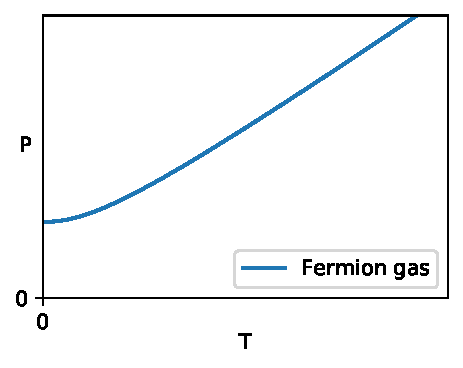
\includegraphics[width=0.65\textwidth]{figs/week09_pressure.pdf}\end{center}

\vspace{24 pt}
\begin{center}\textbf{More information about supernovas and relativistic fermions \\ will be added over the weekend.}\end{center}
% ------------------------------------------------------------------



% ------------------------------------------------------------------
\newpage
\subsection{Type-Ia supernovas}


% even though white dwarfs are quite hot by everyday standards, their interior temperatures of roughly $10^7$~K are still very small compared to their Fermi energies that correspond to roughly $01^9$~K. % 0.3MeV~10^5 eV with eV~10^4 K being the Boltzmann constant

% white dwarfs that accrete matter from a companion giant star, leading to a steadily increasing mass. As the white dwarf's mass approaches the Chandrasekhar limit, its central density increases, and, as a result of compressional heating, its temperature also increases. This eventually ignites nuclear fusion reactions, leading to an immediate carbon detonation, which disrupts the star and causes the supernova
% named after \href{https://en.wikipedia.org/wiki/Subrahmanyan_Chandrasekhar}{Subrahmanyan Chandrasekhar}

\TODO{...}

% https://www.esa.int/ESA_Multimedia/Images/2014/09/Artist_s_impression_of_Type_Ia_supernova
These type Ia supernovas play a key role in demonstrating that the expansion of the universe is accelerating (a phenomenon popularly called `dark energy'), which was awarded the 2011 Nobel Prize in Physics.

\TODO{Being written...}
% ------------------------------------------------------------------



% ------------------------------------------------------------------
\newpage
\subsection{Massless fermions}

\TODO{white dwarft Fermi energy around $0.3$~MeV approaching electron mass--energy around $0.5$~MeV...}

\TODO{Being written...}
% ------------------------------------------------------------------
